\documentclass[a4paper, 12pt]{report}
\usepackage[utf8]{inputenc}
\usepackage[T1]{fontenc}

\usepackage{xcolor}
\usepackage{afterpage}

\usepackage{relsize}
\usepackage{moresize}

\usepackage{graphicx}
\usepackage{geometry}


\usepackage{amssymb}
\usepackage{tikz}
\usepackage{amsmath}
\usepackage{textcomp}
\usepackage{eurosym}
\usepackage{systeme}
\usepackage{mathtools}
\usepackage[colorinlistoftodos]{todonotes}
\usepackage[bottom]{footmisc}
\usepackage{mwe}
\usepackage{csquotes}
\usepackage{subfig}
\usepackage{color,soul}
\usepackage{bm}

\newtheorem{theorem}{Theorem}

\usepackage[
    backend=biber,
    style=apa,
  ]{biblatex}

\addbibresource{references.bib}
% [CHANGE] The title of your thesis. If your thesis has a subtitle, then this
% should appear right below the main title, in a smaller font.
\newcommand{\theTitle}{Learning in Social Networks}
\newcommand{\theSubTitle}{}


% [CHANGE] Your full name. In case of multiple names, you can include their
% initials as well, e.g. "Robin G.J. van Achteren".
\newcommand{\theAuthor}{Roman S. Oort}

% [CHANGE] Your student ID, as this has been assigned to you by the UvA
% administration.
\newcommand{\theStudentID}{12189030}

% [CHANGE] The name of your supervisor(s). Include the titles of your supervisor(s),
% as well as the initials for *all* of his/her first names.
\newcommand{\theSupervisor}{A. Haret} % Dr. Ing. L. Dorst

% [CHANGE] The address of the institute at which your supervisor is working.
% Be sure to include (1) institute (is appropriate), (2) faculty (if
% appropriate), (3) organisation name, (4) organisation address (2 lines).
\newcommand{\theInstitute}{
Institute for Logic, Language and Computation\\ %Informatics Institute
Faculty of Science\\
University of Amsterdam\\
Science Park 907 \\ % Science Park 904\\
1098 XG Amsterdam % 1098 XH  Amsterdam
}

% [CHANGE] The date at which you will finalize and submit your thesis.
\newcommand{\theDate}{June 25th, 2021}

\DeclareMathOperator*{\plim}{plim}
\newcommand{\T}{\bm{T}}
\newcommand{\Tij}{\T_{ij}}
\newcommand{\Soc}{(\T(n))^{\infty}_{n=1}}
\newcommand{\beli}[3][2]{p_{#2}^{(#3)}}
\newcommand{\belvec}[2]{\bm{p}^{(#2)}}

\begin{document}
%\pagestyle{empty}
% Page I

% This page should contain your title and name and will create a thumbnail
% which should be readable at https://scripties.uba.uva.nl/



    \newgeometry{margin=1cm}
    \thispagestyle{empty}
    
    % [CHANGE]
    % You can also use one of the other background colors, 
    % preferably one that fits with your cover-image
    % see https://en.wikibooks.org/wiki/LaTeX/Colors for suggestions
    \pagecolor{black}\afterpage{\nopagecolor}
 
    \begin{minipage}[t][0.8\paperheight]{0.8\paperwidth}
        \begin{center}
        
                  %% Print the title a at the top in white.
                  {\color{white} \fontsize{52}{104}\selectfont \textbf{\theTitle} }
               
                  \vspace{0.2\paperheight}
                  
                  % [CHANGE]
                  % Replace this image with one that is relevant for your research, 
                  % If possible, use one of your own illustrations
                 
                  
\includegraphics[width=0.75\paperwidth]{ThesisKI/UvAThesisLayout/augmented-intelligence.jpeg}
                  
                   %% Print the author at the bottom 
                  \vspace{0.2\paperheight}
                  
                 {\color{white} \fontsize{24}{48}\selectfont \textbf{\theAuthor} }
        \end{center}
    \end{minipage}   
   
    \restoregeometry
    
\newpage

% Page II
\thispagestyle{empty}
\newgeometry{margin=1cm}
\vspace*{0.8\textheight}
\noindent
Layout: typeset by the author using \LaTeX. \\
Cover illustration: Unknown artist 
\restoregeometry

\newpage
\thispagestyle{empty}
% Page III
\begin{center}

\vspace{2.5cm}


\begin{Huge}
% see definition at beginning of document
\theTitle
\end{Huge} \\

\vspace{0.5 cm}

\begin{Large}
\theSubTitle
\end{Large}

\vspace{1.5cm}

% see definition at beginning of document
\theAuthor\\
% see definition at beginning of document
\theStudentID

\vspace{1.5cm}

% [DO NOT CHANGE]
Bachelor thesis\\
Credits: 18 EC

\vspace{0.5cm}

% [DO NOT CHANGE] The name of the educational programme.
Bachelor \textit{Kunstmatige Intelligentie} \\
\vspace{0.25cm}

\includegraphics[width=0.075\paperwidth]{ThesisKI/UvAThesisLayout/uva_logo.png} \\
\vspace{0.1cm}

% [DO NOT CHANGE] The address of the educational programme.
University of Amsterdam\\
Faculty of Science\\
Science Park 904\\
1098 XH Amsterdam

\vspace{2cm}

\emph{Supervisor}\\

% see definition at beginning of document
\theSupervisor

\vspace{0.25cm}

% see definition at beginning of document
\theInstitute

\vspace{1.0cm}

% see definition at beginning of document
\theDate

\end{center}
\newpage

\thispagestyle{empty}

\tableofcontents

\thispagestyle{empty}

\newpage

\pagenumbering{arabic}
\setcounter{page}{1}

\addtocontents{toc}{\protect\thispagestyle{empty}}

\chapter{Introduction}

\chapter{Literature Review}
\section{Social Learning}
Social learning is a field of study used in various different disciplines, ranging from Economy to Psychology, concerning the beliefs of agents in groups, and how these beliefs evolve and change over time \parencite{reed2010sociallearning}. Research in this field is dedicated to determining how individuals, and groups as a whole, change their beliefs and actions based on beliefs and actions of those around them. Many models have been proposed to formalize this process \parencite{golub2017learning}, with the DeGroot model being one of the most prominent \parencite{degroot1974concensus}.

\section{DeGroot Model}
\subsection{Agent Interaction}
\label{interaction:matrix}
The DeGroot model \parencite{degroot1974concensus} consists of a set of $N=\{1, 2, ..., n\}$ of agents, interacting and exchanging information, at discrete time-steps, and an $n \times n$ \emph{interaction} matrix $\T$ describing the nature of these interactions, representing a \emph{social network}. This interaction matrix describes to whom each agent in the network listens, and to which extent. An element $\Tij > 0$ of the interaction matrix indicates that agent $i$ listens to agent $j$, and the value of this entry determines how much weight agent $i$ places on agents $j$'s opinion: the higher this value, the more important $j$'s opinion is to $i$. It is important to note that $\T$ is a positive matrix, meaning it is not possible for an agent to place a negative weight on another agents opinion, but that they are ever only capable of ignoring other agents, or agreeing with them in some manner. 

\newpage

\noindent Furthermore, the weight matrix $\T$ is assumed to be row-stochastic, meaning that the elements along its rows sum to one:
\begin{align*}
    \sum_{j=1}^{n} \Tij = 1.
\end{align*}

\noindent Finally, $\T$ is not necessarily symmetrical, making it entirely possible for an agent $i$ to hold the opinion of agent $j$ in high regard, while in return $j$ thinks very little of $i$'s opinion, or not even anything  at all.

\noindent Besides the interaction matrix, the model also contains a belief vector, $\bm{p}$, which will be elaborated on in the following section.

\subsection{Belief \& Learning}
\label{beliefs}

The belief of an agent $i \in N$, at a discrete time $t \in \{0, 1, 2, ...\}$, is denoted as $p_{i}^{(t)}$, where this belief is taken as a real number in the interval $[0, 1]$. At the start of the process, at $t=0$, each agent $i$ is given a personal belief, through a private signal:
\begin{align*}
    \beli{i}{0} = \mu + e_i,
\end{align*}
where $\mu$ is a real number, again on the interval $[0, 1]$, assumed to be the truth, and $e_i$ is an error term for agent $i$, independently and identically distributed, with zero mean.
The beliefs of all agents are recorded into the belief vector $\bm{p}^{(t)}$, where the $i$'th entry corresponds to the belief of agent $i$, at time $t$.

\noindent As time progresses the agents in the network update their own belief based on the beliefs of the agents around them, using the following updating rule:
\begin{equation}
    \label{updating:standard}
    \bm{p}^{(t)} = \T\bm{p}^{(t-1)}.
\end{equation}
In other words, in order to obtain the belief vector at time $t$, the belief vector at $t-1$ can be matrix multiplied with the interaction matrix representing the network. This makes the updating step for a single agent simply the weighted sum of its neighbours' opinions, where $i$'s neighbours are those agents that $i$ listens to, as follows:
\begin{align*}
    \beli{i}{t} = \sum_{j=1}^{n}\Tij\beli{j}{t-1},
\end{align*}

\newpage

\noindent Furthermore, it is possible to compute the belief vector $\bm{p}^{(t)}$, without computing the belief vector at every preceding $t^\prime < t$, the formula for which can be derived from Equation \ref{updating:standard}, as follows:
\begin{align*}
    \bm{p}^{(t)} &= \T\bm{p}^{(t-1)} \\
    &= \T\T\bm{p}^{(t-2)}\\
    &= \T^2\bm{p}^{(t-2)}\\
    &= \T^3\bm{p}^{(t-3)} \\
    & \ \ \ \ \ \  \vdots \\
    &= \T^{t}\bm{p}^{(0)}.
\end{align*}
In other words, the belief vector at time $t$ can be computed by multiplying the interaction matrix $\T$ with itself $t$ times, and multiplying the resulting matrix with the initial belief vector.


\subsection{Convergence}
\label{convergence}
As we are interested in the spread of information through the network, and whether or not the agents in a network will learn the supposed true state of the world, an important notion is the concept of \emph{convergence}. The interaction matrix $\T$ is said to be convergent if:
\begin{equation*}
    \lim_{t\to\infty} \T^t\bm{p},
\end{equation*}
exists for all $\bm{p} \in [0, 1]^n$. That is to say, as time progresses sufficiently, the beliefs of the agents, independent of their starting signal, approach a constant value and no longer change.

\noindent In order for a network to exhibit convergence, there are several properties of networks that play an important role, the first being \emph{aperiodicity}, which is a necessary condition for convergence. Aperiodicity is a property that concerns the cycles in a network, that is to say, paths that start and end at the same node, or in this context, agent. In order for a network to be aperiodic the greatest common divisor of the length of \emph{all} cycles in the network can be no larger than one \parencite{degroot1974concensus}. This can be ensured as long as one agent in the network has a self-link, as this would create a cycle of length one.

\noindent Another notion important in the convergence of social networks is \emph{connectedness}. When applied to undirected networks, wherein an edge between two agents works both ways, a network is said to be connected when there exists some path between any two agents $i$ and $j$. However, when applied to \emph{directed} networks this property changes slightly, and can be divided in two distinct notions. More specifically, a connected directed network can be either \emph{weakly} or \emph{strongly} connected. A directed network is said to weakly connected if there exists some undirected path between any two agents in the network. However, if there also exists a \emph{directed} path between any two agents, a directed network is said to be strongly connected.

\noindent Now, with the aforementioned concepts the following theorem can be stated made \parencite{degroot1974concensus}:

\begin{theorem}
\noindent Assuming that $\T$ is the row-stochastic interaction matrix of a strongly connected network, the following three statements are equivalent:
\begin{itemize}
    \item[-] $\T$ is convergent
    \item[-] $\T$ is aperiodic
    \item[-] There is some unique left eigenvector, $\bm{s}$, of $\T$, corresponding to the eigenvalue $\lambda=1$, such that, for every $\bm{p}\in [0,1]^n$, and every agent $i$,
    \begin{align*}
        (\lim_{t\to\infty}\T^t\bm{p})_i = \bm{sp}
    \end{align*}
\end{itemize}
\end{theorem}

 \noindent This last eigenvector property not only provides a definition of convergence, but also the actual convergent belief of the network, which is nothing more than a multiplication of the left eigenvector, also called the influence vector, $\bm{s}$ and the belief vector $\bm{p}$. Furthermore, as $\bm{s}$ is a $1 \times n$ row-vector, and $\bm{p}$ an $n \times 1$ column-vector, their multiplication results in a single number, highlighting that there is one single, universal, convergent belief.

\newpage

\subsection{Wisdom of Crowds}
\label{wisdom}
Having established the convergence property for social networks it becomes possible to look towards the notion of wisdom, central in \parencite{golub2010naive}. They defined wisdom to mean that a given network not only converges, but converges to the assumed true state of the model, $\mu$, specifically in the context of large societies. That is to say, as the size of the network $n\to\infty$ the convergent belief tends towards the assumed truth $\mu$.

\noindent To encapsulate the idea of large societies, providing insight in the behaviour of these models as the participating number of agents becomes sufficiently large, limiting statements with regard to the number of agents are used. To this end a society is defined as a sequence of networks, indexed by the number of agents in the network, $n$: $\Soc$. This means that the entry $\textbf{T}(n)$ is the interaction matrix of the network in the sequence with $n$ agents, where $\textbf{T}(n)_{ij}$ is used to denote the entry $(i,j)$ in this specific sequence. Said method of indexing is applied to all properties of these networks, e.g.: belief vectors, influence vectors.

\noindent The beliefs of the agents are generated using the same mechanism described in Section \ref{beliefs}, i.e.: independently and identically distributed zero mean error terms added to the assumed truth. The belief of an agent $i$ at a time $t$ is denoted as $\beli{i}{t}(n)$, in a network with $n$ agents. Under the assumption that every network in the given sequence converges, the convergent belief of an agent $i$, that is to say the belief as $t \to\infty$, as described in Section \ref{convergence}, is denoted as $\beli{i}{\infty}(n)$.

\noindent Using these notations a sequence $\Soc$ is deemed to be wise if:
\begin{equation*}
    \label{wisdom:equation}
    \plim_{n\to\infty}\max_{i \leq n}|\beli{i}{\infty}(n) - \mu| = 0,
\end{equation*}
That is to say, a sequence of network is wise if, as $n$ becomes sufficiently large, the convergent belief of \emph{every} agent in the network is equal to the truth, which, using the fact that the convergent belief can be computed using the influence vector $\bm{s}$, can be rewritten as:
\begin{equation*}
    \label{wisdom:influence}
    \plim_{n\to\infty} \textbf{s}(n)\bm{p}^{(0)}(n) = \mu,
\end{equation*}
which holds if and only if $s_{1}(n) \to 0$, where $s_1(n)$ is the first entry in the \emph{ordered} influence vector $\bm{s}$. Simply put, a sequence of networks if wise if and only if the influence of the most influential agent tends to zero, as $n$ becomes sufficiently large.

\newpage

\section{Obstructions to Wisdom}
While the wisdom of crowds effect is a powerful notion, it is not infallible. Most notably, it is also a fragile concept, with many factors capable of disrupting the network's ability to obtain wisdom. Some of these factors are consequences of the structure of the networks, while other are caused by agents that do not cooperate, and stick to their opinion no matter what.

\subsection{Prominent Families}

One such obstacle is a natural extension of the vanishing influence condition mentioned previously. Just as how a single agent cannot hold too much sway over the network, the same holds for \emph{groups} of agents in a network. The influence of a group $B$ on another group $C$ is simply defined as the sum of all weight placed on all agents $i \in B$ by all agents $j \in C$. 

\noindent Another way to measure the influence of a group is using that group's \emph{t-step prominence}, which looks at the group's influence in relation to the entirety of the network rather than in relation to a single other group. More specifically, the \emph{t-step prominence} of a group $B$ at a given time $t$, is simply the lowest weight placed by any agent $i \notin B$ on any agent $j \in B$.

\noindent However, as we are interested in sequences of networks, we need to extend the definition of groups into sequences as well. Therefore we define a family to be a sequence of groups $(B_n)$ in the network, such that each $B_n \subset \{1, ..., n\}$.

\noindent Now, a family is capable of preventing the wisdom of a network. If a finite family is exists that, for every network in the sequence, for some $t$, has a t-step prominence larger than some constant $\alpha$, this family will prevent the network from being wise.


\subsection{Non-cooperative Agents}
\label{non-coop}

Another factor capable of preventing wisdom, and whose influence is also the main subject of the thesis, are non-cooperative agents in the network. That is to say, an agent that does not adhere to the updating mechanics, like all other agents, but instead sticks to its initial opinion, no matter what \parencite{amir2021robust}. It is also important to note that, while these non-cooperative agents do not follow the updating procedure, they still share their opinion to their neighbouring agents. This causes the presence of only one of these non-cooperative agents to be enough to not only prevent the network from becoming wise, but also for every other opinion to adopt the opinion of this non-cooperative agent at the time of convergence \parencite{amir2021robust}. \footnote{Assuming that the non-cooperative agent's opinion does not equal the assumed truth.}



\section{Variations}

As mentioned in Section \ref{non-coop} the presence of non-cooperative agents in the network is greatly disruptive for the ability of a network to achieve wisdom. So much so even, that only one non-cooperative agent is sufficient to prevent any network, regardless of size, from attaining wisdom. Furthermore, not only does this agent prevent wisdom, they also ensure that the final convergent belief of the network will be their own belief, with regard for neither the initial beliefs of the cooperative agents, nor the assumed truth of the network. As the presence of even one such agent disrupts the wisdom of the entire network research is done on how to make the standard, \emph{naive}, DeGroot model more resilient to the presence of such non-cooperative agents. Several variations of the DeGroot model, and how they distinguish themselves from the standard model, will be discussed.

\subsection{$\varepsilon$-DeGroot}

One such variation, specifically designed by \parencite{amir2021robust} to combat the presence of such non-cooperative agents in the network, is called $\varepsilon$-DeGroot. This variation makes a small adjustment to the standard updating rule of the DeGroot model, in an attempt to achieve wisdom, despite any non-cooperative agents present in the network.

\noindent Under the regular DeGroot mechanics an agent updates their opinion simply to the weighted average of their neighbouring agents' opinion, $y_i$, regardless of how far this weighted average deviates from their current opinion. In contrast, the $\varepsilon$-DeGroot mechanics employ a threshold, given by the parameter $\varepsilon$. Should the difference between an agent's current opinion and their new opinion, $y_i$, exceed this threshold, the agent will update their belief to the closest of $\{y_i - \varepsilon, y_i + \varepsilon\}$. However, in the case that the difference does not exceed the threshold, the agent will revert to their previous belief, held at $t-2$. The updating rule for an agent $i$ at time $t$ is therefore changed to the following:

\begin{equation*}
    \label{edegroot:updating}
  \beli{i}{t} =\Bigg\{
  \begin{matrix*}[l]
  y_i, \text{ if } |\beli{i}{t-2} - y_i| \leq \varepsilon\\
  y_i^{\prime}\in\{y_i-\varepsilon, y_i+\varepsilon\}\text{ s.t. }|\beli{i}{t-2} - y_i^{\prime}|\text{ is minimized, otherwise}
  \end{matrix*}
\end{equation*}

\noindent Therefore, the larger $\varepsilon$ is chosen, the more an agent can change their opinion in a single updating step, and the smaller this $\varepsilon$ is chosen, the less an agent will change their opinion. It is important to note that this updating rule achieves a somewhat different form of convergence that \parencite{amir2021robust} call \emph{alternating convergence}. This means that, rather than having a single convergent belief vector, a network whose agents update their opinion in accordance with this rule will have \emph{two} convergent belief vectors, alternating between time-steps.

\subsection{Private Belief}

Another variation introduced by \parencite{friedkin1990private}, permits each agent to hold on to persistent private belief. When updating, each agent will not only consider the weighted sum of the beliefs of their neighbouring agents, but also take into account this private belief. Furthermore, this private belief does not change over time, but remains constant, making it distinct from an agents' link to themselves, should this self-link be present. After all, a self-link only considers the currently held belief, which changes at every step. This variation on the model changes the updating rule to the following:

\begin{equation*}
    \beli{i}{t} = (1-\alpha_i)y_i + \alpha_i b_i,
\end{equation*}

\noindent where $b_i \in [0, 1]$ is the private belief of an agent $i$, and $\alpha_i \in [0, 1]$ is the weight that said agent places on their private belief, and $y_i$ weighted sum of its neighbours' opinions, computed as under regular DeGroot mechanics. In essence the updating rule becomes a weighted sum of the new belief, as computed through the standard updating rule, and an agent's private belief.
 
\newpage
\chapter{Method}
\section{Network Generation}

\subsection{Random Generation}
\label{generation:random}

In order to examine the behaviour of the DeGroot dynamics we created a function \texttt{generate\_network}, to generate \emph{random} networks, to ensure the generality of the obtained results. This function, and all others, were programmed in Python 3.9.2. For the computation and implementation of the network structure the \emph{NumPy} \parencite{2020NumPy-Array} and \emph{SciPy} \parencite{2020SciPy-NMeth} packages were used, and the visualizations were created using a combination of the \emph{Matplotlib} \parencite{matplotlib} and \emph{NetworkX} \parencite{networkx} packages. Furthermore the \texttt{generate\_network} function accepts several parameters in order to shape the network generation process as desired.

\subsubsection{Default Case}
In the default, most basic, case the \texttt{generate\_network} function simply takes the desired number of agents, $n$ as input. Other, optional, parameters can be provided to customize the desired network and will be discussed in detail at the relevant time. To start, an empty $n\times n$ array,  that is to say an array containing only zeroes, is created, serving as a blank slate for the interaction matrix $\T$ of the network. 

\noindent Subsequently the function will iterate over the agents in the network, starting at the first and ending at the $n$'th agent, adding edges to every agent, in order to ensure the generated network is fully connected at every size. 

\noindent In this iteration there is one special case, namely, the very first agent. To ensure aperiodicity, as discussed in [REF], and therefore convergence, the very first agent is guaranteed to receive a self-link. As this creates a cycle of length one, aperiodicity is guaranteed, as then there can no longer be a common denominator greater than one for \emph{all} cycles in the network. We want our network to be aperiodic as, according to Section \ref{wisdom} we assume all networks in the sequence to be convergent in order for a sequence to be wise, and, as seen in Section \ref{convergence}, an aperiodic network is also convergent.

\noindent After the first agent, every subsequent one will have both an incoming and outgoing edge, when generating a directed network. When generating an undirected network each agent is guaranteed to have one edge, which is both incoming and outgoing. This guarantees that the network of size $n$ will be fully connected. 

\noindent However, we need to generate a sequence of networks, where every network is strongly connected, not only the network of size $n$. To that end, when generating these guaranteed edges for an agent $i$, the agent $j$ on the other end of these edges is chosen randomly randomly, from a uniform distribution, out of all agents already present in the network before $i$ was added. As can be seen in Section \ref{proof:conn}, when generating a network of size $n$, this network is also strongly connected at every size $n^{\prime} < n$.

\noindent Therefore, as this method of generation not only guarantees connectedness in the total network, but also at every smaller size of the network, this returned network can also be considered a sequence of networks. To access a network of a specific size in this sequence, one would only need to take the rows and columns up to that size to obtain the specific network. This ensures that the network and its links stay constant between sizes, allowing for proper comparison of different networks in the sequence. 

\noindent Finally, this function is also capable of growing an existing network: when a matrix and a positive integer $m$ are provided, the function will grow this existing matrix by adding $m$ rows and columns, one for each agent, whose links are determined in the same way as described earlier.

\noindent We favour this method of network generation over other, more standard methods, for several reasons. Most importantly, implementing the network generation from scratch provides more low-level control over the network generation process, allowing more options for customization. A clear effect is the strong connectedness mentioned earlier. Using another method for generating the network, while possibly faster when initially generating the network, would require another pass over all agents to ensure the network is fully connected, and remains so at every size. 

\newpage

\noindent Another, more subtle, effect of the chosen method is a slight bias towards the earlier agents in the network, an effect which can be seen in Figure \ref{degree:agent}, showing the degree for the average the degree for every 100 agents added consecutively to the network. As shown earlier the agents are added to the network the higher their degree tends to be. This mirrors how those individuals who are part of a group for a long time tend to have more connection than those new to the group.

\begin{center}
    \begin{figure}[!htbp]
        \centering
        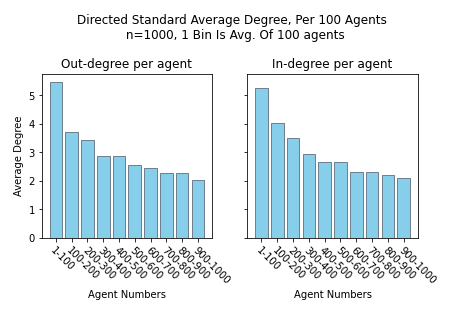
\includegraphics[width=.8\textwidth]{ThesisKI/Images/DirectedStandardPerAgent.png}
        \caption{Average Degree per 100 agents}
        \label{degree:agent}
    \end{figure}
\end{center}
\newpage
\subsubsection{Parameters}

As mentioned in Section \ref{generation:random} the \texttt{generate\_network} function has several parameters to steer the generation procedure in the desired direction, allowing to change the degree, the amount of neighbours of an agent, and the probability of a self-link, among others. 

\noindent First of all, the \texttt{directed} parameter controls whether the generated network is directed or undirected. By default the generated networks are directed, meaning that an edge is only either incoming or outgoing. However, when the \texttt{directed} parameter is set to \texttt{False}, an edge is both incoming and outgoing. Therefore, where a directed network had two guaranteed edges for each agent, one incoming and one outgoing, an undirected network will have only one edge, functioning as both an incoming and outgoing edge.

\noindent Secondly, the optional parameter \texttt{increase\_degree} allows each agent to have more than the links guaranteed by the default generation process, as outlined in Section \ref{generation:random}. This is done by generating an additional degree for each agent, which is randomly sampled real number from a given distribution, by default a normal distribution with mean two and a standard deviation of one, rounded to the nearest integer. Then, a corresponding amount of agents is chosen randomly from the \emph{entire} set of $n$ agents, instead of only the preceding agents, using a uniform distribution.

\noindent The difference between these two methods can be seen in Figures \ref{deg:std} and \ref{deg:inc}, showing the degree distribution for a default network and a network with increased degree respectively. As seen in Figure \ref{deg:std}, in an undirected network with the default degree, nearly half of the agents will only have the minimum degree.\footnote{In the network used to generate Figures \ref{deg:std} and \ref{deg:inc} each agent had a self-link, which leads to a minimum degree of two when combined with the guaranteed edge.} Furthermore, the tail of the distribution quickly dissipates. However, when the degree is increased using the \texttt{increase\_degree} parameter, the distribution is flattened and more equally spread out, as seen in Figure \ref{deg:inc}: the highest peak consists of only two hundred agents and the lower peaks show a much more gradual decline in frequency, compared to the default generation.
\begin{figure}[!htbp]
  \centering
  \subfloat[Standard Degree]{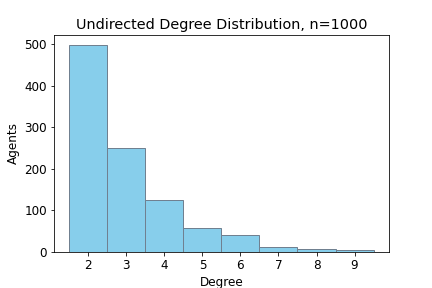
\includegraphics[width=0.5\textwidth]{ThesisKI/Images/DegreeUndirectedStd.png}\label{deg:std}}
  \hfill
  \subfloat[Increased Degree]{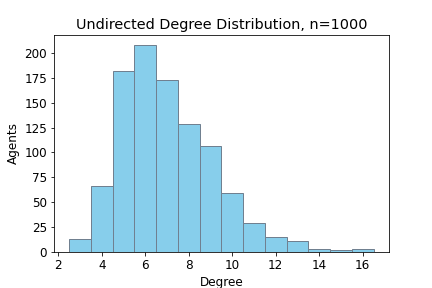
\includegraphics[width=0.5\textwidth]{ThesisKI/Images/DegreeUndirectedInc.png}\label{deg:inc}}
  \caption{Degree Distributions Undirected Network}
\end{figure}

\noindent A final parameter is \texttt{p\_selflink}, which determines the probability for each agent to have an edge to (and from) itself. When set one, every agent in the network will receive and edge to themselves and, conversely, when set to zero, no agent in the network will have an edge to themselves, with the exception of the very first agent, to ensure aperiodicity, as mentioned in Section \ref{generation:random}.

\noindent A final parameter  for the customization of the network generation is the probability of a self-link, which can be set at the moment of generation. This sets the probability for each agent to form a link with itself, save for the first agent, which always receives a self-link in order to ensure the aperiodicity of the network.
\begin{center}
    \begin{figure}[!htbp]
        \centering
        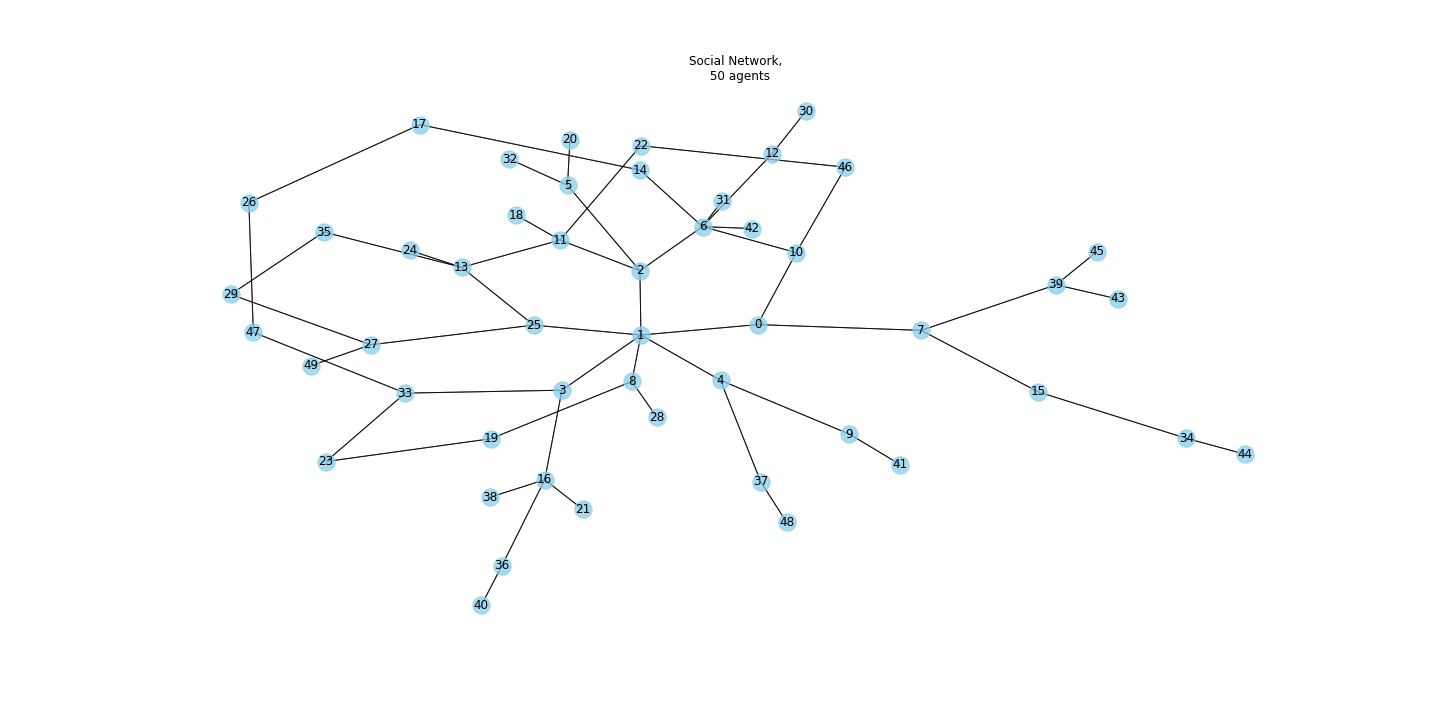
\includegraphics[width=1.1\textwidth]{ThesisKI/Images/NoneGraphRandom.png}
        \caption{Example of Randomly Generated Undirected Network}
        \label{network:random}
    \end{figure}
\end{center}

\newpage

\subsubsection{Sparse Matrices}

One challenge of the chosen implementation is the memory consumption. As the interaction matrix is two-dimensional, its memory consumption increases in a polynomial manner with respect to the number of agents. As the wisdom of crowds effects occurs as the network size increases towards infinity this poses a problem, with large networks consuming large amounts of memory. In order to circumvent this problem the implementation of the network generation stores the interaction matrix in a sparse format \parencite{2020SciPy-NMeth}. As can be seen in Figure \ref{generation:memory} this decreases the memory consumption to negligible levels, for networks of up to $10,000$ agents, whereas when using a standard, dense, matrix the memory consumption increases rapidly. \newline
However, generating a network as a sparse matrix is a somewhat slower process than generating the same network as a dense matrix, though both generation processes still run in linear time as can be seen in Figures \ref{generation:time_inc} and \ref{generation:time_std},  which show the network generation times for a network with increased degree, and standard degree respectively. Therefore, as the generation of the network needs only be run once, the decrease in memory usage was considered to outweigh the slightly increased run-time, and the sparse generation was chosen as default.
\begin{figure}[!htbp]
    \centering
    \subfloat[]{\label{generation:memory}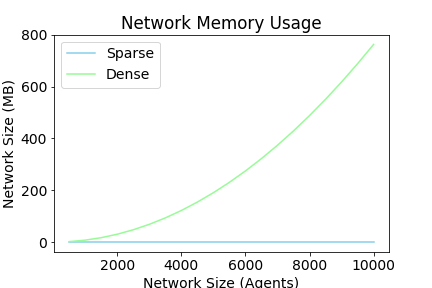
\includegraphics[scale=.4]{ThesisKI/Images/Memory.png}}
    
    \begin{minipage}{.45\linewidth}
    \centering
    \subfloat[]{\label{generation:time_inc}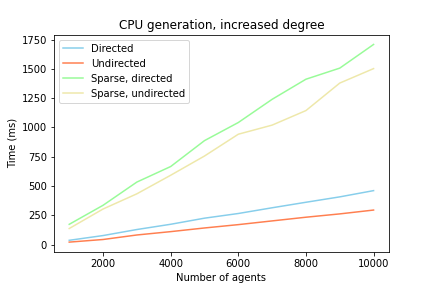
\includegraphics[scale=.35]{ThesisKI/Images/CPU_inc.png}}
    \end{minipage}%
    \begin{minipage}{.45\linewidth}
    \centering
    \subfloat[]{\label{generation:time_std}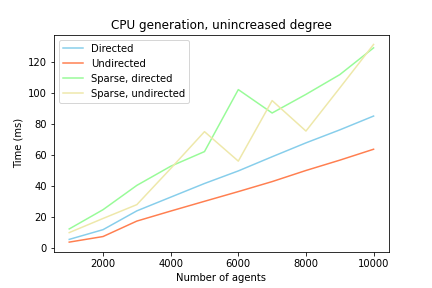
\includegraphics[scale=.35]{ThesisKI/Images/CPU.png}}
    \end{minipage}\par\medskip
    \caption{Network generation, \\ memory and time consumption}
\end{figure}

\newpage
\subsection{Belief Generation}

The generation of the beliefs follows the procedure as discussed in section [REF]. That is to say, the initial opinion of an agent $i$, $\beli{i}{0}$, is generated by adding a random, independently sampled, zero-mean, error term, $e_i$, to the assumed truth of the network. This is implemented by generating an array of length $n$, where each entry is sampled from a zero mean probability distribution, $\mathcal{N}(0, 0.75)$ by default. The assumed truth, $\mu$, is drawn randomly from a uniform distribution on the interval $[0, 1]$, and is added to each entry in this array of error terms. \newline
However, as mentioned in section [REF] all beliefs are to lie on the interval $[0, 1]$, which is not guaranteed with this method. After all, as $\mu$ is chosen randomly it can lie arbitrarily close to the edges of the interval, allowing for the a very small error term to push the belief outside of the interval. What's more, the probability distribution is continuous, meaning it is even possible for an error term to be larger than $1$.  Therefore, in order to force each belief onto this interval the initial belief vector is value normalized, according to following rule:
\begin{equation*}
    \beli{i, \text{norm}}{0} = \frac{\beli{i}{0} - \min(\bm{p}^{(0)})}{\max(\bm{p}^{(0)}) - \min(\bm{p}^{(0)})},
\end{equation*}
which ensure that the smallest belief in the belief vector is normalized to $0$, the highest belief normalized to $1$, and every other belief will fall somewhere in between. However, as this shift the mean of the belief vector away from $\mu$, $\mu$ itself must undergo the same normalization in order to ensure each belief is still properly generated from this value.
\newline

\subsection{Weight Initialization}
The \texttt{generate\_network} function in Section \ref{generation:random} instantiate the network by creating the edges between the agents. However, it does not yet place a weight on all of these links, to describe how much value agents assign to the beliefs of others. For this purpose different options to initialize the weights have been determined. These are all applied only on the non-zero entries in the interaction matrix, therefore they do not create any new links, nor do they remove those already existing links, potentially disrupting the connectedness of the network. 

\noindent Finally, it is important to note that the weight initialization functions do not yet guarantee the interaction matrix to be row-stochastic, as mentioned in Section \ref{interaction:matrix}, therefore the function \texttt{normalize\_weights} was made, which will be discussed in more detail in Section \ref{weights:normalization}

\subsubsection{Uniform}

The first, default, weight initialization is uniform weighting. This simply means that every agent places the exact same weight on the opinions of every other they are connected to. The implementation amounts to simply let the interaction matrix $\T$ remain as is, with a $1$ indicating a link and a $0$ indicating no link.

\subsubsection{Overlap}

The second initialization is based on the idea that an agent prefers to receive information from as many different sources as possible. The weight placed on an agent is therefore proportional to the amount of new information they are able to provide, based on the overlap in neighbours between two agents, where agents' neighbours are those other agents with whom they have a link, denoted as $N_i(n)$. The weight initialization is based on the following rule:
\begin{equation*}
    \T_{ij}(n) = 1 - \alpha \cdot \frac{|N_i(n) \cap N_j(n)|}{|N_i(n)|},
\end{equation*}
This initialization essentially subtracts the fraction of overlap between the set of neighbours of agents $i$ and $j$ from the weight that $i$ places on $j$. This fraction is then multiplied with a discount factor $\alpha \in [0, 1)$ to ensure that a link between agents is not deleted in the event that their neighbouring sets perfectly overlap. 

\subsubsection{Belief}

Another method of setting the weights between agents is based on the idea that agents are more willing to pay attention to those around them with the same mindset. The weight that one agent places on another is based on their difference in opinion: the more similar their opinions the more weight they attribute to the other's opinion, and vice versa. First, in order to set the weights this way, the initial belief vector is concatenated with itself $n$ times, to form an $n \times n$ matrix where each column is the belief vector at $t=0$, as follows:
\begin{equation*}
    B(n) = [\bm{p}^{(0)}(n)]^{n},
\end{equation*}

\noindent In order to get the difference in belief between any two agents, the transpose of the matrix formed by concatenating the belief vectors can simply be subtracted from the matrix itself. Then, for every non-zero element in $\T$, the weight is set as the absolute difference in opinion subtracted from 1, as follows:
\begin{equation*}
    \T_{ij}(n) = 1 - \alpha \cdot |B_{ij}(n) - (B^{T})_{ij}(n)|,
\end{equation*}

\noindent Again, just as in the overlap initialization, $\alpha \in [0, 1)$ is a discount factor to prevent deletion of links, should two connected agents hold perfectly opposed beliefs.

\subsubsection{Random}

Another method of initializing the weights of the network is to simply generate the the weights randomly. This method generates an $n \times n$ matrix filled with numbers sampled from a given distribution, and corresponding parameters, a uniform distribution on $[0, 1]$ by default. In order to ensure the weights are applied only to existing links the randomly generated matrix and the interaction matrix $\T$ are multiplied element-wise, as each element of the $\T$ matrix at this point is either $1$ or $0$.

\subsection{Self-links}

One final factor to account for during weight initialization are the self-links. When using either uniform or random weights everything works as intended. 

\noindent However, when setting the weight based on either overlap of belief unintended behaviour occurs. 

\noindent Namely, when setting the weights based on overlap, a self-link will always be assigned the lowest possible weight. After all, two identical sets, in this case the overlap between the sets of neighbours of agents $i$ and $i$, will perfectly overlap.
Conversely, when setting the weights based on beliefs, a self-link will always receive the highest possible weight. After all, the difference in opinion between an agent and themselves will always be $0$. \newline
In order to circumvent this, when initializing the weights using one of the aforementioned methods, the self-links will be assigned a random weight, sampled from a normal distribution whose mean and standard deviation are taken to be the mean and standard deviation of all other weights in the network. This ensures that the self-links are generated to be more in line with all other weights in the network.

\subsection{Normalization}
\label{weights:normalization}
Finally, in order to achieve convergence, it is necessary that $\T$ is row-stochastic, meaning its elements sum to one, row-wise. In order to ensure this condition, after the weights have been initialized, the matrix is normalized row-wise as follows:
\begin{equation*}
    \T_{ij, norm}(n) = \frac{\T_{ij}(n)}{\sum_{j}\T_{ij}(n)},
\end{equation*}

\noindent In other words, each entry is simply divided by the sum of all weights in the corresponding rows. While this does not preserve the exact values given to the weights by the initialization function, it does preserve their values in relation to the other weights in the row, which is the most important.

\newpage

\subsection{Non-cooperative Agents}

\noindent First it is important to note the representation of non-cooperative agents in the interaction matrix $\T$. We assume a non-cooperative agent to be an agent that does not change its opinion, while still sharing its opinion with their neighbouring agents. They can therefore simply be represented in the matrix as an empty row, save for the element on the diagonal, as this ensures the agent represented by this specific column receives no information from any agent but themselves, causing them to never change their opinion.

\noindent Now, to ensure that the benefits of the \texttt{generate\_network} function, as described in Section \ref{generation:random}, are not lost upon addition of the non-cooperative agents, and to ensure any network in the sequence generated can be made non-cooperative, the non-cooperative agents are not added directly into the network. Rather, for each non-cooperative the agents with whom they share their opinion, who are chosen randomly from all $n$ agents, are saved. Additionally, each non-cooperative agent is guaranteed to receive a link to one of the first five agents on the network, ensuring they will be present in smaller networks, even when their randomly assigned agents all happen to be among the last agents added to the network.

\noindent The links of these non-cooperative agents are then stored to allow them to be added to a network of any size. In order to add them to any network in the sequence, regardless of size, first empty rows are concatenated to the interaction matrix. After all, what distinguishes non-cooperative agents from their cooperative counterparts is their lack of incoming links, expressed by empty rows in the interaction matrix. After the empty rows are added, the respective columns are added, representing those agents who listen to non-cooperative agents. The regular interaction matrix of size $n \times n$ is therefore extended to a matrix of size $(n+m) \times (n+m)$, where $m$ is the number of non-cooperative agents.
An example of a resulting non-cooperative network can be seen in Figure \ref{network:noncoop}, where the non-cooperative agents are labeled in red.

\begin{center}\todo{increase font-size}
    \begin{figure}[!htbp]
        \centering
        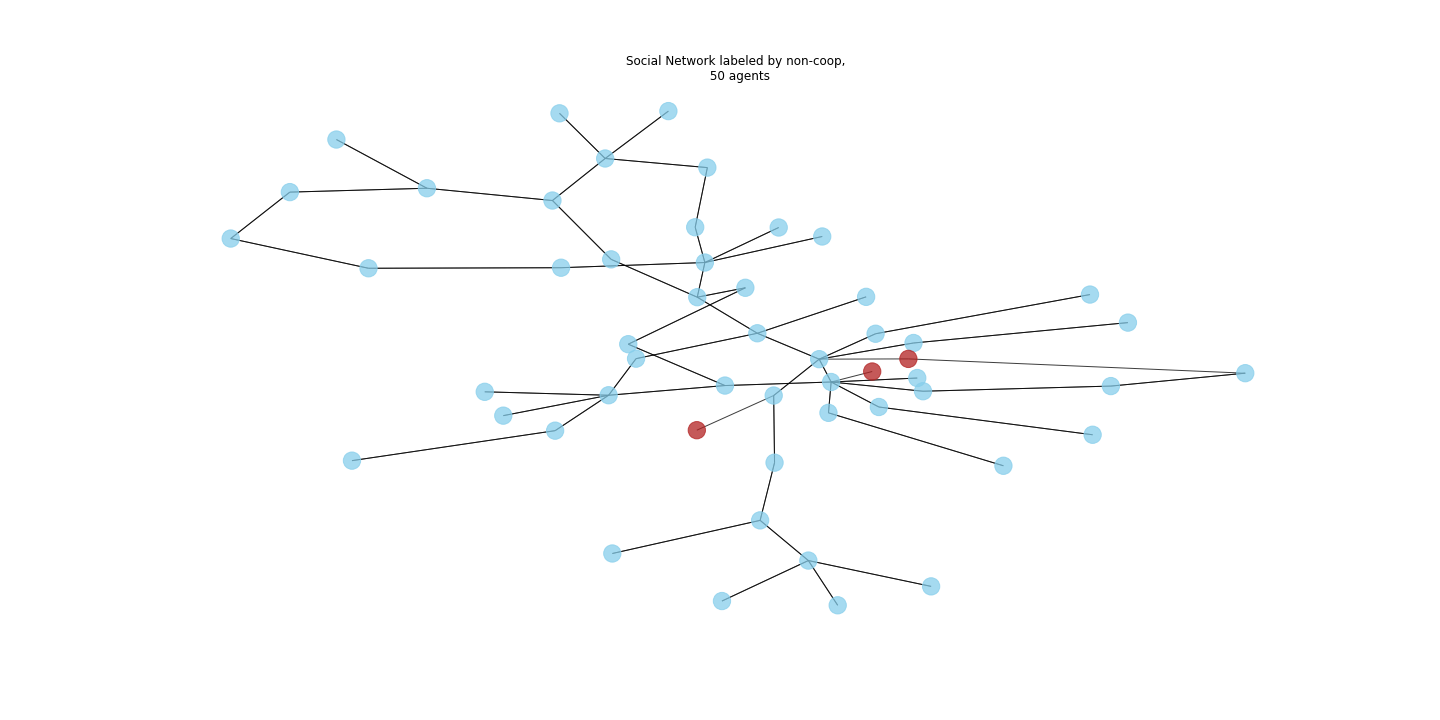
\includegraphics[width=.8\textwidth]{ThesisKI/Images/NonCoopGraph.png}
        \caption{Non-cooperative network, $n=50, m=3$}
        \label{network:noncoop}
    \end{figure}
\end{center}


\newpage


\section{Updating Rules \& Convergence}

In order to compare the different variations on the DeGroot mechanics these variations all needed their respective updating rules to be implemented.

\subsection{DeGroot}

As shown in section [REF]\todo{ref naar updating rule section} $\bm{p}^{(t)}$ can be computed two different ways. The first is the iterative method described in equation [REF] \todo{ref naar iterative updating method}, simply multiplying the belief vector at the previous time-step, $\bm{p}^{(t-1)}$, with the interaction matrix, $\T$, and repeating this process $t$ times. In order to converge a network, using the standard DeGroot dynamics, this process is repeated, until the difference between $\bm{p}^{(t)}$ and $\bm{p}^{(t-1)}$ is zero, or near enough. In other words, the updating step is applied until the beliefs no longer change from one step to another.

The second is to use the method described in equation [REF] \todo{ref naar verkorte updating rule}, which states that to compute the belief vector for a specific $t$, the initial belief vector can be multiplied with the interaction matrix, raised to the power of that $t$. However, upon examination of the computational time, as shown in Figure \ref{update:time}, [REF] \todo{ref naar exponentiation update rule}, is significantly slower, for both dense and sparse matrices.
\todo{fontsize}
\begin{figure}[!htbp]%
    \centering
    \subfloat[\centering Dense Matrix]{{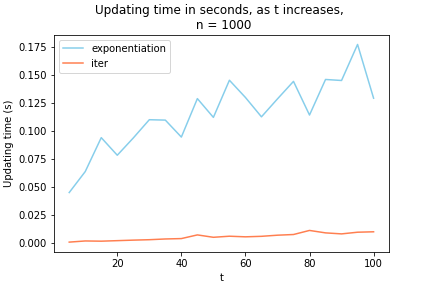
\includegraphics[width=.45\textwidth]{ThesisKI/Images/UpdatingTimeDense.png} }}%
    \qquad
    \subfloat[\centering Sparse Matrix]{{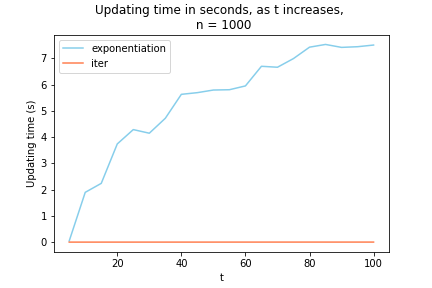
\includegraphics[width=.45\textwidth]{ThesisKI/Images/UpdatingTimeSparse.png} }}%
    \caption{Updating time}%
    \label{update:time}%
\end{figure}

Therefore the iterative method was implemented, in order to significantly speed the updating process. Furthermore, this also allows for saving all intermediate belief vectors, providing insight in the rate of convergence of the network.

However, as shown by \parencite{degroot1974concensus}, the convergent belief can also be computed directly, using the eigenvector of the interaction matrix, $\T$, corresponding to $\lambda=1$. Therefore another function was made for those cases where only the convergent belief is of interest. This function gives only the convergent opinion of the network.

\subsection{$\varepsilon$-DeGroot}
\subsubsection{Standard}

The second updating rule that can be sued to converge a network is the $\varepsilon$-DeGroot variation mentioned in section [REF]\todo{ref naar section $\varepsilon$}. The general framework is the same as for standard DeGroot method: repeatedly apply the updating rule until the beliefs stop changing. However, to converge a network using this method a slight modification is necessary. First of all under the $\varepsilon$-DeGroot dynamics the belief vectors do not adhere to the standard notion of convergence as under regular DeGroot dynamics, rather, using this updating rule results in what \parencite{amir2021robust} describe as \textit{alternating convergence}. That is to say, rather than one single convergent belief vector, there are two convergent belief vectors, between which the agents alternate.
Therefore, using the same condition for convergence as regular DeGroot mechanics will result in an infinite loop, as the belief vectors will alternate, ensuring there will always be a difference between the beliefs at $t$ and $t-1$. To this end, the convergence condition is changed somewhat. Rather than comparing the beliefs between $t$ and $t-1$ only, the belief vectors are compared between $t$ and $t-2$, to check whether their difference is 0, or near enough. This is also done for the beliefs at $t-1$ and $t-3$ to check whether both of the alternating belief vector have converged. As long as convergence has not occurred for both belief vectors the agents the process keeps repeating.

\subsubsection{Alternative}

The alternate $\varepsilon$-DeGroot dynamics work similarly to the standard $\varepsilon$-DeGroot updating rule, as described in [REF] \todo{ref naar alt $\varepsilon$}. Similarly, it also displays \textit{alternating} convergence, rather than the more standard notion of converge. Therefore, in order to properly detect when the network has converged the same conditions for converge are used as with the standard $\varepsilon$-DeGroot mechanics.

\subsection{Private Belief}

Another updating rule implemented allowed each individual agent to account for a private, constant, belief when updating their opinion. In the chosen implementation this private belief was chosen to be the initial belief at time $t=0$. This way agents will always place some amount of weight on their initial belief. The weight placed on this initial belief is specified by the parameter $\alpha \in [0, 1]$. Converging a network using this updating rule, follows the same process as regular DeGroot mechanics, i.e. repeatedly applying the updating rule until the belief vector no longer changes between iterations. As this updating method results in the more standard notion of convergence, opposed to \textit{alternating} convergence, no further modifications to the convergence procedure were required.

\subsection{Threshold}

Another, minor, modification to the regular DeGroot updating mechanics imposes a threshold on the updating rule, ensuring that agents do not drastically change their opinion in a single updating step. Whenever an agent changes their opinion between two time-steps they can change their opinion by no more than the given threshold, effectively limiting how volatile an agents opinion is, simulating a hesitancy in rapid, drastic, changes in opinion.

\newpage

\chapter{Results}
\label{results}

The results in the following section are all obtained from networks randomly generated using the same parameters. More specifically, every generated network is a directed network with an increased degree, where each agent is guaranteed to have self-link. For generating the additional degree the default distribution, as seen in Section [REF], is used.

\noindent Furthermore, the results shown for the standard deviation, distance from the assumed truth and the convergence time, are averaged over ten iterations, in order to obtain more general results. For each of the iterations a new network and initial belief vector was generated, using the same parameters as mentioned above. The graph that shows the convergence of the network towards the truth of the model is simply taken to be the last of these ten iterations.

\noindent Finally, not every updating rule showed uniform convergence. That is to say, the agents did not necessarily adopt the same opinion at the time of convergence for every updating rule. Whenever it was the case that the standard deviation of the belief vector at convergence did not equal $0$, the convergent belief was taken to be the mean of the belief vector.

\newpage

\section{Cooperative Networks}

As can be seen in Figure \ref{coop:compare}, in a cooperative network all updating rule behave quite similar. The convergent belief differs the most for smaller network sizes. However, as the network size increases this difference dissipates, and the convergent beliefs become more and more similar, both to the other updating rules \emph{and} the assumed truth of the model.

\noindent However, while the convergent beliefs are mostly similar, the standard deviation of the convergent belief vector does differ significantly between updating rules. Where the regular and thresholded DeGroot mechanics have no deviation in the convergent belief vector, meaning there is a single convergent belief held by every agent, the other updating rules end up with a non-insignificant amount of variation in the belief vector. This means that, while the agents may no longer update their opinions, their convergent opinions still differ from each other. 

\noindent Finally, the thresholded and regular DeGroot mechanics both reach convergence in the same amount of time, while the other updating rules are significantly faster to reach the point of convergence. However, the standard and thresholded DeGroot mechanics show a clear downward trend in convergence time, which is less present for the other updating rules.

\begin{figure}[!htbp]
    \centering
    \subfloat[]{\label{generation:memory}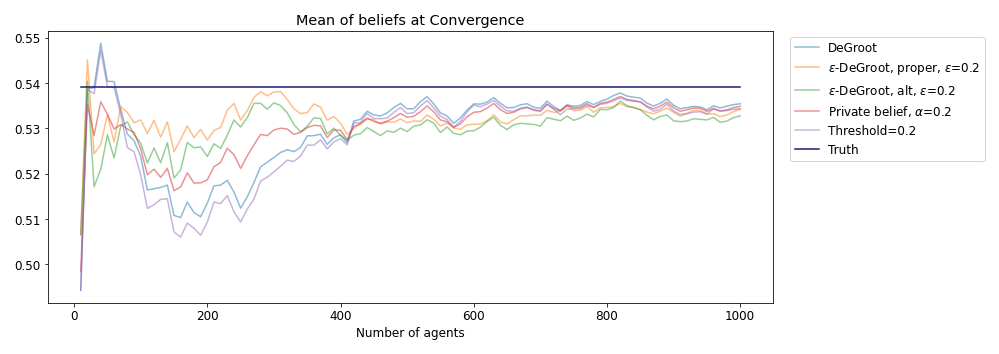
\includegraphics[scale=.45]{ThesisKI/Images/convergence0.png}}
    
    \begin{minipage}{.45\linewidth}
    \centering
    \subfloat[]{\label{generation:time_inc}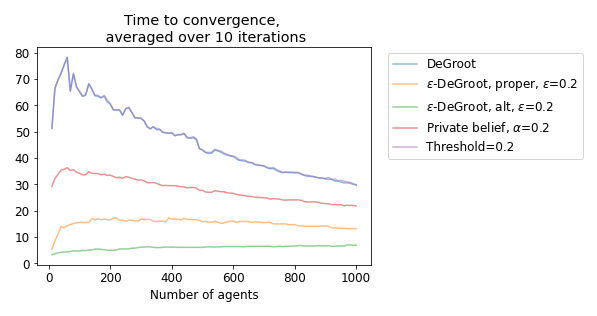
\includegraphics[scale=.4]{ThesisKI/Images/time0.png}}
    \end{minipage}%
    \begin{minipage}{.45\linewidth}
    \centering
    \subfloat[]{\label{generation:time_std}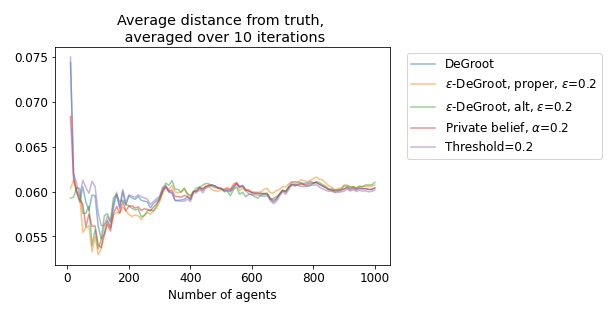
\includegraphics[scale=.4]{ThesisKI/Images/distance0.png}}
    \end{minipage}\par\medskip
    \centering
    \subfloat[]{\label{generation:memory}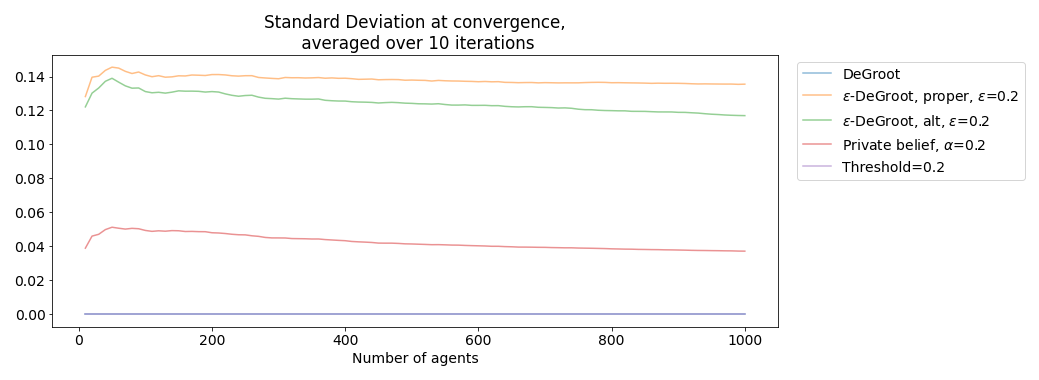
\includegraphics[scale=.45]{ThesisKI/Images/std0.png}}
    
    \caption{Network generation, \\ memory and time consumption}
\end{figure}

\newpage

\section{Non-cooperative networks, $n=1$}

Where the different updating rules behaved in a similar fashion as the regular DeGroot updating mechanics in a fully cooperative network, significant differences start to appear when applied to a network with so much as one non-cooperative agent, as demonstrated in Figure \ref{noncoop1:compare}. 

\noindent First of all, as expected, under regular DeGroot dynamics the convergent opinion becomes that of the non-cooperative agent, and the same applies to the thresholded DeGroot mechanics. Furthermore, again as expected, this belief is uniform, held by every agent in the network, However, the other three updating mechanics exhibit vastly different behaviour. Instead of converging towards the opinion of the non-cooperative agent, the network still converges towards the truth. However, once again, this is not a uniform convergence, as there still is some deviation in the convergent belief vector, though this appears to decline ever so slightly as the network size increases. Furthermore, the standard deviation for the private belief updating rule is somewhat higher when compared to a fully cooperative network Figure \ref{coop:compare}. Also, just as in a cooperative network, the standard deviation of the private belief updating rule is significantly less than that of the $\varepsilon$-DeGroot variations.

\noindent Finally, the updating time for both the regular and the thresholded DeGroot mechanics behave nearly identical, and both display a significant increase in convergence time, whereas the other three updating rules do not appear to show significantly slower convergence. Furthermore, where it decreased as the network grew in a fully cooperative network, the convergence time only increases as the network grows in the presence of a non-cooperative agent. This increase in convergence time can be explained by the presence of the single non-cooperative agent, whose influence has to spread throughout the entire network, taking more and more time to reach every agent as the network size increases. Furthermore, this appears to be a non-factor for the other updating rules, where the non-cooperative agent is not nearly as formative, or even formative at all, for the convergent opinion, making it so that it does not significantly impact the convergence time as a result.

\begin{figure}[!htbp]
    \centering
    \subfloat[]{\label{generation:memory}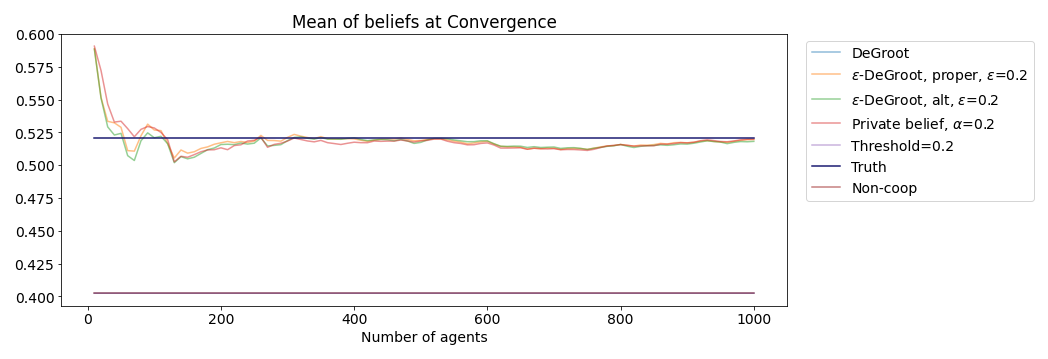
\includegraphics[scale=.45]{ThesisKI/Images/convergence1.png}}
    
    \begin{minipage}{.45\linewidth}
    \centering
    \subfloat[]{\label{generation:time_inc}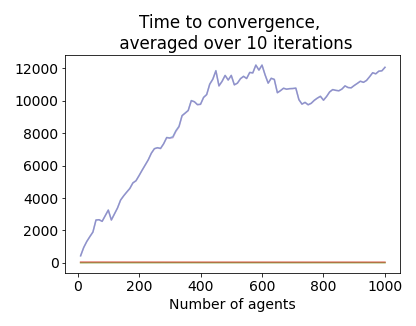
\includegraphics[scale=.4]{ThesisKI/Images/time1.png}}
    \end{minipage}%
    \begin{minipage}{.45\linewidth}
    \centering
    \subfloat[]{\label{generation:time_std}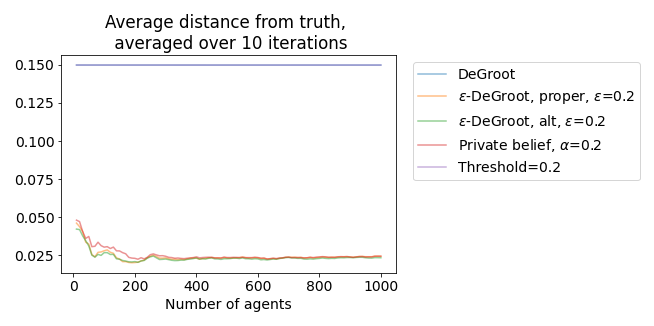
\includegraphics[scale=.4]{ThesisKI/Images/distance1.png}}
    \end{minipage}\par\medskip
    \centering
    \subfloat[]{\label{generation:memory}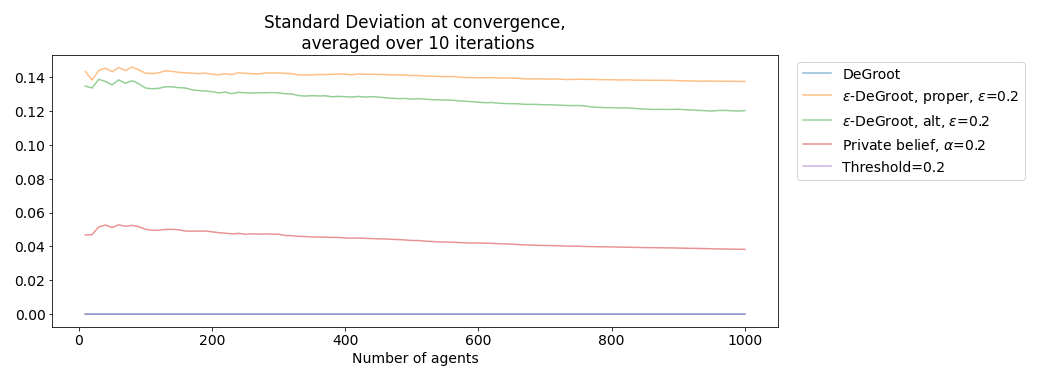
\includegraphics[scale=.45]{ThesisKI/Images/std1.png}}
    
    \caption{Network generation, \\ memory and time consumption}
\end{figure}

\newpage

\section{Non-cooperative networks, $n > 1$}

Finally, in networks with multiple non-cooperative agents there is once again a significant difference in the behaviour of the various updating rules, as seen in Figure \ref{noncoop+:compare}. Once again, both the regular and thresholded DeGroot mechanics converge towards the opinions of the non-cooperative agents, tending towards some, weighted, average between the opinions of those agents, regardless of the assumed truth. However, the effect of these non-cooperative agents is negligible to the convergent belief of the network when using the other three updating rules, all of which still converge towards the assumed truth of the network. 

\noindent However, the regular and thresholded DeGroot mechanics no longer display uniform convergence in the presence of multiple non-cooperative agents, although the standard deviation of the convergent belief vector does decrease quickly as the network size increases. On the other hand, the standard deviation of the convergent belief vector for the other updating rules does not appear to change drastically when additional non-cooperative agents are added to the network

\noindent Finally, while still significantly higher than in a fully cooperative network, the convergence time is shorter than in the presence of only one non-cooperative agent, for both the regular and thresholded DeGroot mechanics. As the number of non-cooperative in the network increases so too does their combined influence, reducing the time it takes for them to influence all cooperative agents. All the other three updating rules are still unaffected in their convergence time, as the influence of the non-cooperative agents on their updating process is very limited.

\begin{figure}[!htbp]
    \centering
    \subfloat[]{\label{generation:memory}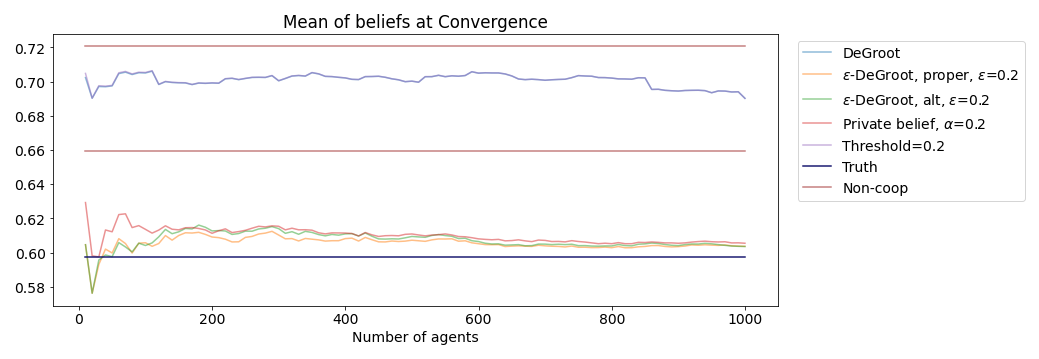
\includegraphics[scale=.45]{ThesisKI/Images/convergence2.png}}
    
    \begin{minipage}{.45\linewidth}
    \centering
    \subfloat[]{\label{generation:time_inc}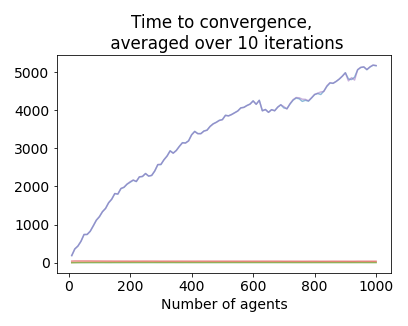
\includegraphics[scale=.4]{ThesisKI/Images/time2.png}}
    \end{minipage}%
    \begin{minipage}{.45\linewidth}
    \centering
    \subfloat[]{\label{generation:time_std}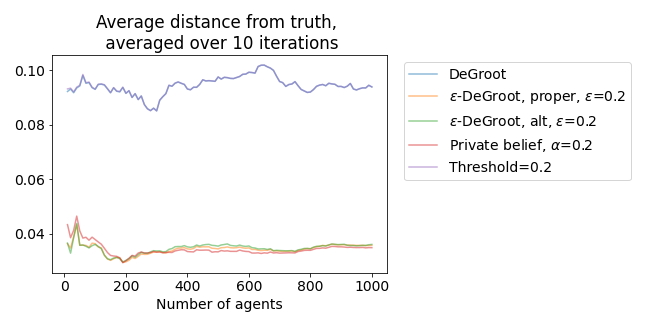
\includegraphics[scale=.4]{ThesisKI/Images/distance2.png}}
    \end{minipage}\par\medskip
    \centering
    \subfloat[]{\label{generation:memory}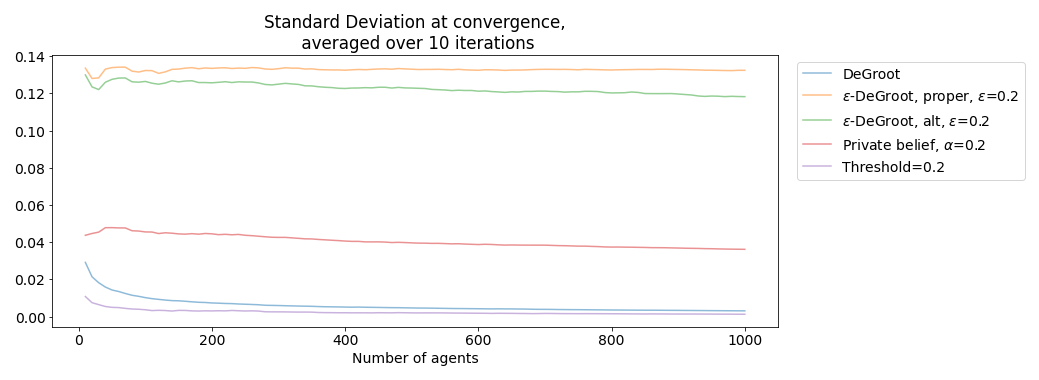
\includegraphics[scale=.45]{ThesisKI/Images/std2.png}}
    
    \caption{Network generation, \\ memory and time consumption}
\end{figure}

\newpage

\chapter{Conclusion and Future Work}
\section{Conclusion}

The goal of the thesis was to examine the behaviour of social networks where agents update their opinions using the DeGroot mechanics, as discussed in Section [REF], and the emergent \emph{Wisdom of Crowds} effect that arises from this updating rule. More specifically, the goal was to examine the influence of any non-cooperative agents, those who refuse to change their opinion, on this effect, and how variations of the updating rule could provide a more robust updating process, more resilient to non-cooperative agents in the network. Five variations on the DeGroot mechanics, described in more detail in Section [REF], were implemented and compared in three different variations of networks; fully cooperative networks, where every agent changes their opinion; non-cooperative networks where there is only one single agent who does not change its opinion; and finally non-cooperative networks with multiple non-cooperative agents. 

\noindent As shown in Section [REF], when the network is fully cooperative the updating rules behave largely similar, all displaying the \emph{Wisdom of Crowds} effect as the network size increases. However, where the regular and thresholded DeGroot mechanics achieve a uniform converge, where every agent holds the same belief at the time of converge, both variations of the $\varepsilon$-DeGroot mechanics and the private belief updating rules do not. Instead of a single convergent belief held by every agent each agent's convergent belief is somewhat different from its neighbours'. However, their average belief still approaches the assumed truth as the network size increases, still achieving the \emph{Wisdom of Crowds} effect, though a somewhat less powerful notion than the regular DeGroot mechanics. Furthermore, the standard deviation of the private belief updating rule is significantly less than that of the $\varepsilon$-DeGroot variations.

\noindent However, strong differences occur when even a single non-cooperative agent is added to the network. Where the regular and thresholded DeGroot mechanics clearly displayed the \emph{Wisdom of Crowds} effect in a cooperative network, this effect is now completely lost. Instead, each individual agent now assumes the opinion of the single non-cooperative agent, at the time of convergence. However, this is where the other updating rules separate themselves. While they still do not achieve uniform convergence, though the variation in final opinions decreases somewhat as the network grows, the average of their belief vector at the time of convergence does not tend towards the belief of the non-cooperative agent. Rather, the \emph{Wisdom of Crowds} effect is still present, though somewhat weakened, as the average of the convergent belief vector comes ever closer to the assumed truth.

\noindent Finally, in the presence of multiple non-cooperative agents, similar results are achieved. Once again, the regular and thresholded DeGroot mechanics tend towards the opinions of the non-cooperative agents, whereas the other updating rules still exhibit the \emph{Wisdom of Crowds} effect. However, instead of one constant belief for the regular and thresholded DeGroot mechanics, the convergent belief seems to vary between different network sizes, towards some weighted average of the opinion of the non-cooperative agents in the network. Furthermore, in the presence of multiple non-cooperative agents, both the regular thresholded DeGroot mechanics no longer attain uniform convergence, though the standard deviation does tend towards $0$ as the network grows. The other three updating rules however, behave similarly in the presence of multiple non-cooperative agents as they did in networks with only one, still displaying the \emph{Wisdom of Crowds} effect, while the opinions of individual agents do still vary.

\noindent All in all, the $\varepsilon$-DeGroot variations and private belief updating mechanics are successful in making social networks more resilient to the presence of non-cooperative agents, where the thresholded DeGroot rule falls short and agents still end up adopting the opinions of the non-cooperative agents. However, these methods are not infallible, as they lose a powerful effect exhibited by the standard DeGroot mechanics. Namely, while these updating rules still converge, it is no longer the case that every agent ends up holding the same opinion, but rather, each agent adopts a somewhat different opinion from the others.

\section{Future Work}

While interesting results have come forward in this thesis there is still room for further work, as it would be desirable to find a variation on the updating rule still providing increased resilience towards non-cooperative agents, while also allowing for (more) uniform convergence.

\noindent One other variation of the DeGroot mechanics would allow the weights of the network to vary over time, which has been discussed in \parencite{chatterjee1977stochastic}. One of the criticisms of the DeGroot model are its rigid weights, which do not change over time. Therefore a variation of the model where the agents can change the weight they place on others' opinions could be a more accurate reflection of the way people change their opinions, and may provide more resilience in the face of non-cooperative agents.

\noindent Furthermore, another way to combat the presence of non-cooperative agents would be to use \textquote{counter non-cooperative agents}. That is to say, non-cooperative agents specifically designed to oppose the already present non-cooperative agents in the network. The information spread by these two kinds of non-cooperative agents could possibly counteract each other, allowing the regular cooperative agents to converge towards a common opinion, and eventually the assumed truth, as the network grows sufficiently large.

\noindent Besides examining different updating rules there is also the option to look at different ways that misinformation is spread throughout a network. Another vulnerability of the \emph{Wisdom of Crowds} effect, besides the non-cooperative agents, is what \parencite{amir2021robust} describe as \emph{distorted monitoring}, where every agents' initial signal is shifted over by some amount $\delta$ from the assumed truth, which can simply be implemented by using a non-zero-mean noise signal when generating the initial beliefs.

\noindent Finally, another possible direction for future work is to examine different variations of the non-cooperative agents. Where they are now represented as agents in the network receiving information from no agents but themselves, several alternatives could also be examined. First of all, a possible variation would be to represent the non-cooperative agents as a periodic influence, rather than a permanent addition to the network. Rather than permanently spreading their own opinion to their neighbours they would only spread this information every set amount of time, either to specific agents or to the network at large. 

\noindent Another natural extension of the non-cooperative agents would be to look at groups of non-cooperative agents, where the agents in this group would only receive information from other in this group while still sending information to other agents outside the group.

\newpage

\printbibliography

\newpage

\chapter{Appendix}
\section{Proof of (strong) connectedness}
\label{proof:conn}
\textbf{Base Case:} \newline
Let $S_1$ be a random social network of 1 agent, generated using the method described in Section \ref{generation:random}.
S is guaranteed to be fully connected, as the first agent in a network always receives a self-link.\newline

\textbf{Induction Hypothesis:}\newline
Let $S_n$ be an arbitrary, strongly connected, randomly generated network, obtained by the method described in Section \ref{generation:random}. Now let $S_{n+1}$ be the network that is obtained by growing the network $S_n$ by one agent. We now want to prove that if $S_{n+1}$ is grown from $S_n$ using the method from Section \ref{generation:random}, $S_{n+1}$ is also strongly connected.\newline

To grow the network $S_n$ by one agent, the agent $n+1$ is added to the network, with two guaranteed links, one incoming and one outgoing. Let the $i$ and $j$ be the arbitrary agents involved in these links, respectively. By the generation procedure outlined in Section \ref{generation:random}, these agents are guaranteed to be present in $S_n$. However, by our induction hypothesis we now that $S_n$ is strongly connected, therefore there exists a directed path from $i$ and $j$ to any other agent in the network. Therefore, as agent $n+1$ has an incoming link from agent $i$, there exists an incoming path from any agent in the network to $n+1$, and, furthermore, as $n+1$ has an outgoing link to agent $j$, there also exists an outgoing path to any agent in the network. Therefore, as there exists a directed path to any agent in the network from agent $n+1$, $S_{n+1}$ must be strongly connected.\newline
Therefore, as $S_n$ and $S_{n+1}$ were arbitrary networks, it must be the case that any network generated using this method must be strongly connected.\newline

\end{document}

\textbf{\noindent One thing to note is that the $\varepsilon$-DeGroot dynamics as described above do not impose a hard, uniform, limit on how much an agent's opinion can change. But rather, this maximum change is determined by the new belief of each agent, and therefore varies from agent to agent. Therefore an alternate approach to the $\varepsilon$-DeGroot dynamics would be to base the new opinion, should the difference between the currently held opinion and the newly computed one exceed the threshold, on the currently held opinion, rather than the newly computed one, changing the updating rule to:
\begin{equation*}
    \label{edegroot:alt}
    \beli{i}{t} =\Bigg\{
    \begin{matrix*}[l]
        y, \text{ if } |\beli{i}{t-2} - y| \leq \varepsilon\\
        x^{\prime}\in\{\beli{i}{t-2}-\varepsilon, \beli{i}{t-2}+\varepsilon\}\text{ s.t. }|y - x^{\prime}|\text{ is minimized, otherwise}
    \end{matrix*}
\end{equation*}
In other words, should the difference between the new opinion and the previous opinion exceed the threshold, $\varepsilon$ is simply added to, or subtracted from, the current opinion, whichever is closest to the belief as computed through the standard updating rule. This imposes a hard limit on how much an agents opinion can change in a single update, namely $\varepsilon$. This hard limit is universal for all agents in the network, instead of varying across different agents as is the case in the regular $\varepsilon$-DeGroot rule.}
